\titledquestion{Break-Even-Analysis}
Four emerging countries are being considered for the establishment of a new production location: Brazil (B), Russia (R), India (I) and China (C). The investment costs are the same in each country, however, the locations differ in terms of the production costs incurred, as shown in the following table:
\begin{table}[htbp]
  \centering
    \begin{tabular}{l|cccc}
    Type of Cost & B & R & I & C \\
    \hline
Fixed Costs/Year & 40,000 & 50,000 &  60,000 & 80,000  \\
Labor Cost/Unit & 7 & 6 & 4 & 2 \\
Material Cost/Unit & 2 & 4 & 1.5 & 0,5 \\
Transportation Cost/Unit & 3.5	& 1.1 & 2	& 1.5 \\
Taxes and Levies/Unit & 4.5 & 0.9 & 2.5 & 4 \\
\end{tabular}
\end{table}

\begin{enumerate}
	\item Graphically illustrate the functional relationships of all locations! What are the critical production quantities?
	\begin{solution}
		Typically, the cost function takes the form:\\
		$K\left(x\right)=f+k\cdot x$\\
		
		The variable cost items here are: Labor costs, material costs, transportation costs, taxes and levies.\\
	This results in the following cost functions for the four emerging markets:\\
		
		$K_B\left(x\right)=40,000+\left(7+2+3.5+4.5\right)\cdot x=40,000+17\cdot x$\\
		$K_R\left(x\right)=50,000+\left(6+4+1.1+0.9\right)\cdot x=50,000+12\cdot x$\\
		$K_I\left(x\right)=60,000+\left(4+1.5+2+2.5\right)\cdot x=60,000+10\cdot x$\\
		$K_C\left(x\right)=80,000+\left(2+0.5+1.5+4\right)\cdot x=80,000+8\cdot x$\\
		
		\uline{Calculation of critical production quantities}
			\begin{enumerate}
				\item [1] First critical output $x_{BR}$ marks transition between emerging markets Brazil and Russia\\
				$K\left(B\right)=K\left(R\right) \Leftrightarrow$\\
				$40,000+17\cdot x_{BR}=50,000+12\cdot x_{BR} \Leftrightarrow$\\
				$x_{BR}=2,000$
				\item [2] Second critical output $x_{RI}$ marks the transition between emerging markets Russia and India\\
				$K\left(R\right)=K\left(I\right) \Leftrightarrow$\\
				$50,000+12\cdot x_{RI}=60,000+10\cdot x_{RI} \Leftrightarrow$\\
				$x_{RI}=5,000$
				\item [3] Third critical output $x_{IC}$ marks the transition between the emerging markets of India and China\\
				$K\left(I\right)=K\left(C\right) \Leftrightarrow$\\
				$60,000+10\cdot x_{IC}=80,000+8\cdot x_{IC} \Leftrightarrow$\\
				$x_{IC}=10,000$\\
			\end{enumerate}
		\begin{center}
			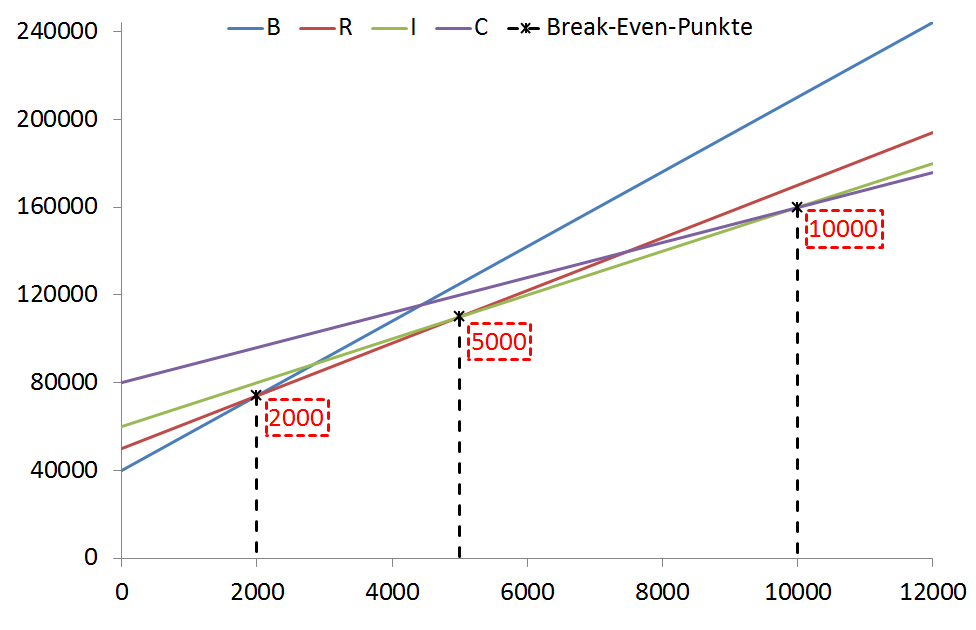
\includegraphics[scale=0.5]{Uebungen/figures/Break_Even_Analyse}\\
		\end{center}
	\end{solution}
	\item What assumptions did you implicitly make in setting up the these cost functions?
	\begin{solution}
	
		\uline{Assumptions of the Break-Even Analysis:}
			\begin{itemize}
				\item Output x is homogeneous (only true for ``single-product companies'').
				\item Linearity of cost functions (e.g. ``experience curve'')
				\item Purely static analysis
			\end{itemize}
	\end{solution}
\end{enumerate}

\ifprintanswers
\else
\newpage
\fi